\documentclass[a4paper,12pt]{amsart}

\usetheme[progressbar=frametitle]{metropolis}
\metroset{block=fill}

\subtitle{NTIN071 Automata and Grammars}
\author{Jakub Bulín (KTIML MFF UK)}

\date{Spring 2025\\ 
    \vspace{1in} 
    \begin{flushleft}
        \it \footnotesize * Adapted from the Czech-lecture slides by Marta Vomlelová with gratitude. The translation, some modifications, and all errors are mine.
    \end{flushleft}
}

%% packages

\usepackage{amsmath}
\usepackage{amssymb}
\usepackage{amsthm}
\usepackage{cancel}
\usepackage{color}
\usepackage{colortbl}
\usepackage{forest}
\usepackage[utf8x]{inputenc}
\usepackage{multicol}
\usepackage{multirow}

%% colors
\definecolor{Gray}{gray}{0.9}

%% TikZ
\usepackage{tikz}
    \usetikzlibrary{
        automata,
        arrows,
        backgrounds,
        decorations.pathmorphing,
        fit,
        positioning,
        shapes,
        shapes.geometric,
        tikzmark
    } 
    \tikzset{>=stealth',shorten >=1pt,auto,node distance=2cm}
    \tikzset{initial text={}}
    \tikzset{elliptic state/.style={draw,ellipse}}

%% amsthm
\theoremstyle{plain}
    \newtheorem*{algorithm}{Algorithm}    
    \newtheorem*{observation}{Observation}
    \newtheorem*{proposition}{Proposition}

\theoremstyle{remark}
    \newtheorem*{exercise}{Exercise}
    \newtheorem*{remark}{Remark}

%% macros
\DeclareMathOperator{\RegE}{RegE}
\DeclareMathOperator{\RL}{RL}

% Just for Lecture 2
\newcommand{\x}{$\times$}
\newcommand{\nx}{\ }


\begin{document}

\thispagestyle{empty}

\section*{NTIN071 A\&G: Tutorial 5 -- Regular expressions (bonus: 2-way automata)}

\medskip

\subsection*{Teaching goals:} The student is able to

    \begin{itemize}\setlength{\itemsep}{0pt}
        \item define regular expressions and the matching languages
        \item construct a regular expression for a language given in set notation
        \item convert a regular expression to a finite automaton
        \item convert a finite automaton to a regular expression
    \end{itemize}

\medskip

\section*{In-class problems}


\medskip\begin{problem}[Constructing regular expressions]

    Find regular expressions representing the following languages over $\Sigma = \{a, b\}$ consisting of words that:

    \begin{multicols}{2}

        \begin{enumerate}[(a)]\setlength\itemsep{0pt}
            \item start with `abba',
            \item start with `ab' and end with `ba',
            \item contain `abba' or `bab' as a subword,
            \item do not contain `aa' as a subword,
            \item contain an even number of a's,
            \item the first letter is the same as the last.
        \end{enumerate}

    \end{multicols}

\end{problem}


\medskip\begin{problem}[Regex to automaton]

    Construct NFAs recognizing the languages described by the following regular expressions:
    
    \begin{multicols}{3}
    
        \begin{enumerate}[(a)]\setlength\itemsep{6pt}
            \item $a^2 + b^2 + ab$
            \item $a + b^*$
            \item $(ab + c)^*$
        \end{enumerate}
    
    \end{multicols}
    
\end{problem}


\medskip\begin{problem}[Automaton to regex]
    
    Construct regular expressions for languages recognized by the following automata.

    (a) 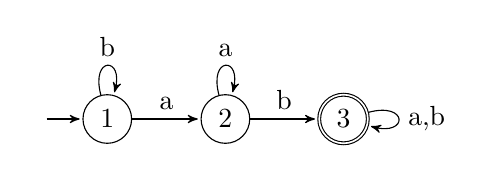
\begin{tikzpicture}[>=stealth',shorten >=1pt,auto,node distance=1.5cm,baseline=(current bounding box.center)]
        \tikzset{every state/.style={minimum size=0.2cm}}                    
        \node[initial,state]  (a1)      {1};
        \node[state] (b1)  [right of=a1]    {2};
        \node[state,accepting] [right of=b1](c1)      {3};
        \path[->]
            (a1)  edge  node {a} (b1)
            (a1)  edge[loop above]  node {b} (a1)
            (b1)  edge  node {b} (c1)
            (b1)  edge[loop above]  node {a} (b1)
            (c1)  edge[loop right]  node {a,b} (c1)
        ;
    \end{tikzpicture}
    \hspace{1.5cm}
    (b)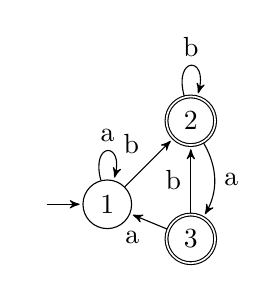
\begin{tikzpicture}[>=stealth',shorten >=1pt,auto,node distance=1.5cm,baseline=(current bounding box.center)]
        \tikzset{every state/.style={minimum size=0.2cm}}
        \node[initial,state]  (a1)      {1};
        \node[state,accepting] (b1)  [above right of=a1]    {2};
        \node[state,accepting] [below of=b1](c1)      {3};
        \path[->]
            (a1)  edge  node {b} (b1)
            (a1)  edge[loop above]  node {a} (a1)
            (b1)  edge[bend left]  node {a} (c1)
            (b1)  edge[loop above]  node {b} (b1)
            (c1)  edge  node {a} (a1)
            (c1)  edge  node {b} (b1)
        ;
    \end{tikzpicture}        

\end{problem}


\medskip\begin{problem}[Complement of a Regular Expression]
    
    Consider the following regular expression over the alphabet $\Sigma=\{a,b\}$ and let $L=L(R)$.
    \[
        R=((a + b)(a + b))^*ab
    \]
    \begin{enumerate}[(a)]
        \item Construct a \emph{nondeterministic} finite automaton $A$ (as small as possible) recognizing $L$.
        \item Use the subset construction to convert $A$ to a \emph{deterministic} finite automaton $B$.
        \item From the automaton $B$, construct a DFA $C$ recognizing the \emph{complement} of $L$.
    \end{enumerate}

\end{problem}

\medskip

\section*{Extra Practice and Thinking}


\begin{problem}[Regex to automaton]

    Construct finite automata accepting languages described by the following regular expressions:
    
    \vspace{-10pt}

    \begin{multicols}{2}
    
        \begin{enumerate}[(a)]\setlength\itemsep{0pt}
            \item $ab + ba$
            \item $((ab + c)+a(bc)^* + b)^*$
            \item $((ab + c)^*a(bc)^* + b)^*$
            \item $(01^* + 101)^*0^*1$
        \end{enumerate}
    
    \end{multicols}
    
\end{problem}


\begin{problem}[Automaton to regex]
    
    Construct regular expressions for languages accepted by the following automata.

    \vspace{-9pt}
    
    \begin{multicols}{2}
        \begin{enumerate}[(a)]
            \item 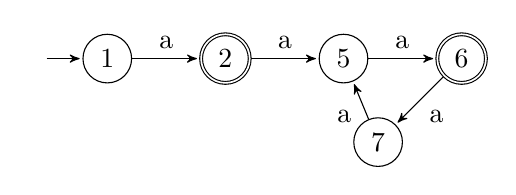
\begin{tikzpicture}[>=stealth',shorten >=1pt,auto,node distance=1.5cm,baseline=(current bounding box.north)]
                \tikzset{every state/.style={minimum size=0.2cm}}
                \node[initial,state]  (a1)      {1};
                \node[state,accepting] (b1)  [right of=a1]    {2};        
                \node[state] (c1)  [right of=b1]    {5};
                \node[state,accepting] (d1)  [right of=c1]    {6};
                \node[state] (e1)  [below left of=d1]    {7};
                \path[->]
                    (a1)  edge  node {a} (b1)
                    (b1)  edge  node {a} (c1)
                    (c1)  edge  node {a} (d1)
                    (d1)  edge  node {a} (e1)
                    (e1)  edge  node {a} (c1)
                ;
            \end{tikzpicture}

            \item 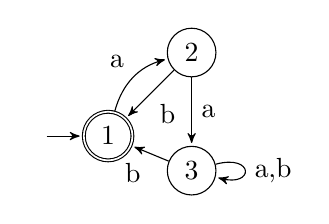
\begin{tikzpicture}[>=stealth',shorten >=1pt,auto,node distance=1.5cm,baseline=(current bounding box.north)]
                \tikzset{every state/.style={minimum size=0.2cm}}
                \node[initial,state,accepting]  (a1)      {1};
                \node[state] (b1)  [above right of=a1]    {2};
                \node[state] [below of=b1](c1)      {3};
                \path[->]
                    (a1)  edge [bend left] node {a} (b1)
                    (c1)  edge[loop right]  node {a,b} (c1)
                    (b1)  edge  node {a} (c1)
                    (b1)  edge  node {b} (a1)
                    (c1)  edge  node {b} (a1)
                ;
            \end{tikzpicture}

            \item 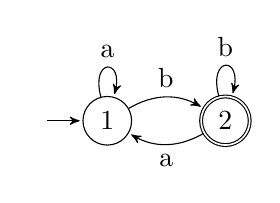
\begin{tikzpicture}[>=stealth',shorten >=1pt,auto,node distance=1.5cm,baseline=(current bounding box.north)]
                \tikzset{every state/.style={minimum size=0.2cm}}			
                \node[initial,state]  (a1)      {1};
                \node[state,accepting] (b1)  [right of=a1]    {2};
                \path[->]
                    (a1)  edge[bend left]  node {b} (b1)
                    (a1)  edge[loop above]  node {a} (a1)
                    (b1)  edge[bend left]  node {a} (a1)
                    (b1)  edge[loop above]  node {b} (b1)
                ;
            \end{tikzpicture}

            \item 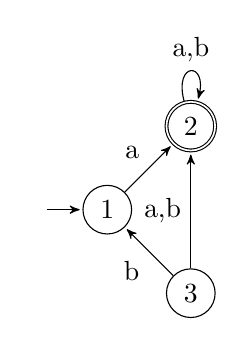
\begin{tikzpicture}[>=stealth',shorten >=1pt,auto,node distance=1.5cm,baseline=(current bounding box.north)]
                \tikzset{every state/.style={minimum size=0.2cm}}
                \node[initial,state]  (a1)      {1};
                \node[state,accepting] (b1)  [above right of=a1]    {2};
                \node[state] [below right of=a1](c1)      {3};
                \path[->]
                    (a1)  edge  node {a} (b1)
                    (b1)  edge[loop above]  node {a,b} (b1)
                    (c1)  edge  node {b} (a1)
                    (c1)  edge  node {a,b} (b1)
                ;
            \end{tikzpicture}
        \end{enumerate}
    \end{multicols}

\end{problem}

\vspace{-12pt}
\begin{problem}[Testing equivalence of regular expressions] 
    
    Describe an algorithm to test equivalence of two regular expressions. Apply it to $(a + b)(a + b)^*$ and $a(a + b)^* + b(a + b)^*$.
    
\end{problem}


\begin{problem}[Are regular expressions regular?]

    Fix a finite alphabet $\Sigma$. Is the language consisting of all regular expressions over $\Sigma$ a regular language?

\end{problem}


\section*{Bonus: Two-way automata}

\begin{problem}[Convert a 2-way automaton]

    Consider the following two-way DFA.

    \vspace{-9pt}

    \begin{multicols}{3}

        \begin{enumerate}[(a)]\setlength{\itemsep}{0pt}
            \item Determine the language it recognizes.
            \item Determine the functions $f_w$ and the congruence $\sim$ for all $w$ of length $\leq 4$.
            \item Convert it to an equivalent one-way automaton.
        \end{enumerate}

        \vspace{-24pt}
        \begin{center}
            \begin{tabular}{ r | c c }
                & a & b \\
                \hline
                $\to\ast p$ & $p,1$ & $q,-1$ \\
                $q$ & $r,1$ & \\
                $r$ & & $p,1$
            \end{tabular}
        \end{center}

        \begin{center}
            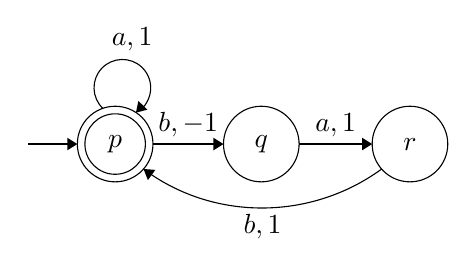
\begin{tikzpicture}[scale=0.16]
                \tikzstyle{every node}+=[inner sep=0pt]
                \draw [black] (10.1,-9.7) circle (3);
                \draw (10.1,-9.7) node {$p$};
                \draw [black] (10.1,-9.7) circle (2.4);
                \draw [black] (21.7,-9.7) circle (3);
                \draw (21.7,-9.7) node {$q$};
                \draw [black] (33.5,-9.7) circle (3);
                \draw (33.5,-9.7) node {$r$};
                \draw [black] (3.2,-9.7) -- (7.1,-9.7);
                \fill [black] (7.1,-9.7) -- (6.3,-9.2) -- (6.3,-10.2);
                \draw [black] (9.129,-6.874) arc (226.70189:-61.29811:2.25);
                \draw (11.45,-2.35) node [above] {$a,1$};
                \fill [black] (11.75,-7.21) -- (12.66,-6.97) -- (11.94,-6.28);
                \draw [black] (13.1,-9.7) -- (18.7,-9.7);
                \fill [black] (18.7,-9.7) -- (17.9,-9.2) -- (17.9,-10.2);
                \draw (15.9,-9.2) node [above] {$b,-1$};
                \draw [black] (24.7,-9.7) -- (30.5,-9.7);
                \fill [black] (30.5,-9.7) -- (29.7,-9.2) -- (29.7,-10.2);
                \draw (27.6,-9.2) node [above] {$a,1$};
                \draw [black] (31.254,-11.682) arc (-53.92224:-126.07776:16.054);
                \fill [black] (12.35,-11.68) -- (12.7,-12.56) -- (13.29,-11.75);
                \draw (21.8,-15.26) node [below] {$b,1$};
            \end{tikzpicture}
        \end{center}

    \end{multicols}

\end{problem}


\begin{problem}[Without 2-way automata this is hard]

    Given a DFA $A$, design an NFA recognizing the language $L'=\{\#w\#\ |\ ww^R\in L(A)\}$. ((Do not use two-way DFAs.)

\end{problem}

\begin{problem}[Constructing 2-way automata]

    Let $L$ be a regular language over $\Sigma$ and $\#\notin\Sigma$. Construct a two-way finite automaton accepting the given language: 

    (a) $L' = \{\#w\#\mid ww^R \in L\}$ \hfill (b) $L' = \{\#w\#\mid (\exists u \in\Sigma^*)( wu \in L\ \wedge \ |w|=|u|)\}$

\end{problem}


\end{document}
